\documentclass[10pt,bibliography=totocnumbered,listof=totocnumbered, footsepline, headsepline]{scrreprt}
\usepackage[a4paper,top=2.5cm,left=2.5cm,bottom=2cm,right=2cm]{geometry}
\usepackage[english]{babel}
\usepackage[utf8]{inputenc}
\usepackage{amsmath}
\usepackage{mathtools}
\usepackage{amsfonts}
\usepackage{amssymb}
\usepackage{amstext}
\usepackage{graphicx}
\usepackage{tabularx}
\usepackage{setspace}
\usepackage[right]{eurosym}
\usepackage{subfig}
\usepackage[usenames,dvipsnames]{color}
\usepackage{colortbl}
\usepackage{array}
\usepackage{parskip}
\usepackage[right]{eurosym}
\usepackage[pdfpagelabels=true]{hyperref}
\usepackage{listings}
\usepackage[automark]{scrlayer-scrpage}
\usepackage{multicol}
\usepackage{float}
\usepackage{enumerate}
\usepackage{pgfplots}
\usepackage{xcolor}
\usepackage{todonotes}
\usepackage{fontawesome}
\usepackage{pdfpages}
\usepackage{fontawesome}

\lstset{ %
	backgroundcolor=\color{white},   % choose the background color
	basicstyle=\footnotesize,        % size of fonts used for the code
	breaklines=true,                 % automatic line breaking only at whitespace
	captionpos=b,                    % sets the caption-position to bottom
	commentstyle=\color{ForestGreen},    % comment style
	escapeinside={\%*}{*)},          % if you want to add LaTeX within your code
	keywordstyle=\color{blue},       % keyword style
	stringstyle=\color{BurntOrange},     % string literal style
}

\definecolor{codegreen}{rgb}{0,0.6,0}
\lstdefinestyle{mystyle}{
    backgroundcolor=\color{black},
    basicstyle=\ttfamily\footnotesize\color{codegreen},
}

% Header Footer
\pagestyle{scrheadings}
\automark[section]{chapter}
\clearscrheadfoot
\ihead[]{TDDI08 and TDTS07 - Embedded Systems Design}
\ohead[]{Traffic Light Simulation}
\ifoot[]{Simon Burkhardt (simbu448), Jule Enninghorst (julen905)}
\ofoot[]{\thepage}
\addtolength{\footskip}{-4ex}
% Section Deapth
\setcounter{secnumdepth}{4}

%\setcounter{section}{2}
\renewcommand{\thesection}{\arabic{section}}
\renewcommand\thefigure{\arabic{figure}}

\renewcommand{\arraystretch}{1.2}


\begin{document}

\title{TDTS07/TDDI08 lab 1 - SystemC}
\author{Simon Burkhardt (simbu448)\\ Jule Eninghorst (julen905)}
\maketitle

\section{Our Approach}
    \subsection{Components}
    
    \begin{figure*}[h]
    	\centerline{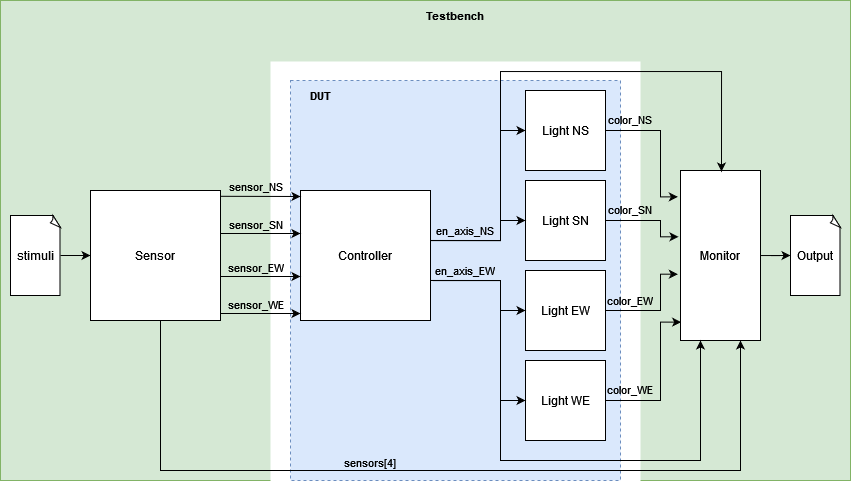
\includegraphics[width=.9\textwidth]{testbench_flowchart.png}}
    	\caption{Testbench, modules and signals of the full traffic light system}
    	\label{fig:Controller_Diagram}
    \end{figure*}
    
    \paragraph*{Sensor} The input for the traffic light system is one file consisting of four columns where each column represents one sensor for each direction at the traffic crossing (NS, SN, EW, WE). The values for the sensor can either be \texttt{1} (a vehicle detected) or \texttt{0} (no vehicle detected). Each row in the file is representing one second. \\
    There is no feeback in the sensor where cars disappear when the light is green. 
    We decided to model the sensors in our system as simple electromagnetic detectors for vehicles. Hence, we only have the two states of a waiting or not waiting car. There is no way of counting how many vehicles are waiting in line as we are only interested in \textit{if} there is a car still waiting and not how many cars are waiting. Furthermore, there is no feedback in the generated traffic. This means that vehicles can disappear without ever being given a green light. We decided to model our system this way, as we believe in a realistic traffic light modeling there could also be bicycles that suddenly disappear as they move onto the sidewalk once they are standing in front of a red traffic light.\\
    %The system furthermore does not care, if a vehicle suddenly disappears e.g. if there is a car waiting at a red light, but disappears without ever turning green (this could be a bicycle changing from the road to the sidewalk).\\
    The \textit{Sensor} class reads the input file and writes the values each second in the corresponding channels of \texttt{sensor\_NS}, \texttt{sensor\_SN}, \texttt{sensor\_EW} and \texttt{sensor\_WE}.
    
    \paragraph*{Controller} These channels signal in which direction the cars are waiting for the \textit{Controller}, which is the core of the traffic light model. Its main purpose is to schedule both axes \texttt{NS} and \texttt{EW} in a fair way.
    That is, in the worst case scenario, where many cars are waiting at each stop light, the scheduler will alternate between the two axes according to a specific timeout value that we set to \texttt{10}s. This aims to avoid that a stop light remains blocked when the other direction has a lot of cars. A state machine for the controller is illustrated in Figure \ref{fig:Controller_FlowChart}. Via the output channels \texttt{en\_axis\_NS} and \texttt{en\_axis\_EW} the controller notifies the other components what axis is enabled or disabled. Where \texttt{1} is enabled (green light allowed) and \texttt{0} is disabled (must be red).
    
    \begin{figure}[H]
    	\centerline{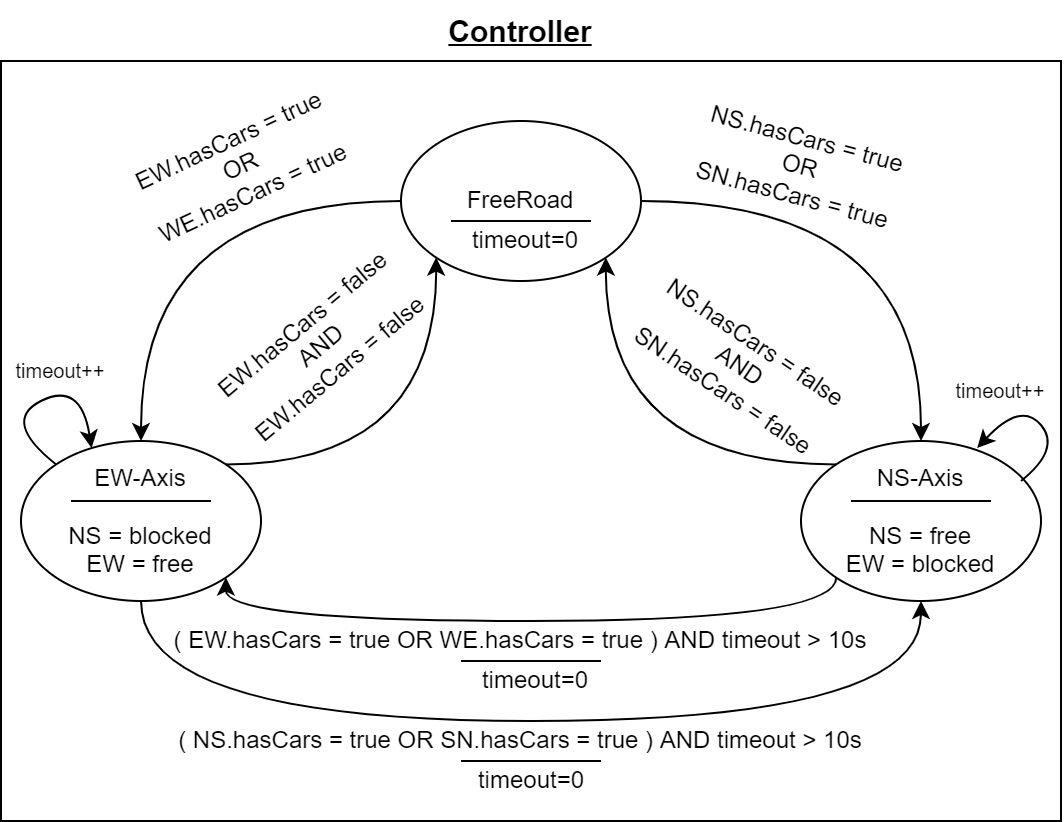
\includegraphics[width=34pc]{Controller_Diagram.drawio.png}}
    	\caption{State machine for the controller logic}
    	\label{fig:Controller_FlowChart}
    \end{figure}
    
    \paragraph*{Light} The \textit{Light} class models the functionality of an individual stop light.
    It has a boolean sensor input to be aware of any waiting cars and a boolean road input to know if the corresponding axis is enabled or not. If both, cars are waiting and the axis is enabled, the stop light writes a green light (\texttt{255}) on the output channel \texttt{color}. Else a red light is written (\texttt{0}).
    The light therefore is an independent piece that can be instantiated as an object.
    
    \paragraph*{Monitor} The last component is the monitor, which checks the given constraints and confirms the validation of the simulation via an output file (more detailed explanation on how to read the results are given in Subsection \ref{subsec:results}). The monitor is not a process with a sensitivity list but a process running at 10x the speed of the controller. This is important to guarantee that the constraints are always satisfied and not only if a signal changes. Thereby the monitor is able to catch errors if a signal is not changing if it should. To check constraints, the monitor views the channels of the color for each traffic light, the sensors signalizing arriving cars as well as the status of the two axes as an input.
    
    \paragraph*{Testbench} The testbench is built in a similar way to a VHDL testbench, which contains the component instances and port map to the different signals.
    The assertions inside the monitor make this testbench \textit{self-checking}. It therefore knows the above design constraints and if any of them is violated, a visual error is produced (as shown in Fig. \ref{fig:assertion_failed}). The process thereby reports errors itself without the need for an engineer having to look at debug files.
    
    \begin{figure}[H]
    	\centerline{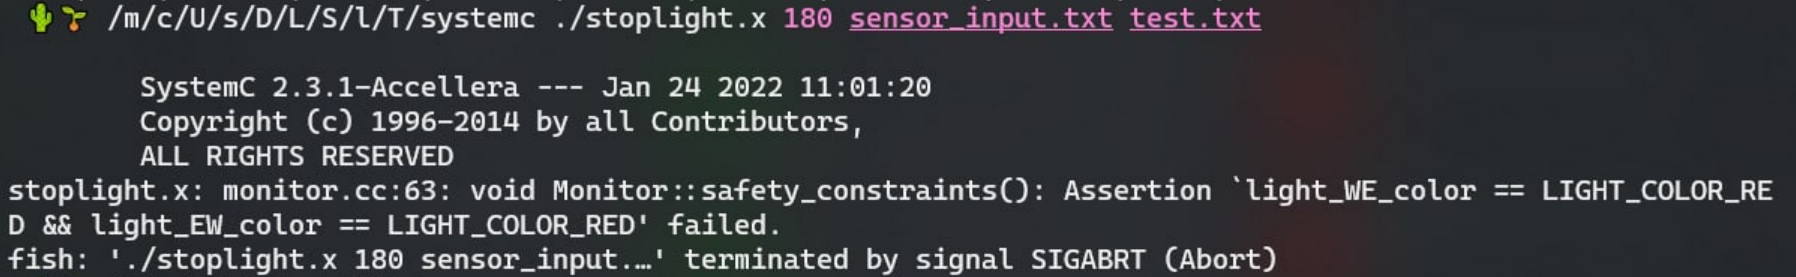
\includegraphics[width=38pc]{assertion_failed.png}}
    	\caption{Failed Assertion when running the simulation where a NS/SN light was green at the same time a EW/WE light was green.}
    	\label{fig:assertion_failed}
    \end{figure}
    
    
    
    
    \subsection{Constraints and System Assumptions}
        \paragraph*{Safety Constraint}
        The most important constraint is, that there must never be a case, where the intersecting axes have a green light at the same time. We therefore introduce a channel for each axis (\texttt{en\_axis\_NS} and \texttt{en\_axis\_EW}) that controls the enabling of the axis and ensures that traffic lights on the different axes are never on green at the same time. To check that this constraint is satisfied by our system the monitor, on the one hand, examines that (\texttt{en\_axis\_NS} and \texttt{en\_axis\_EW}) are never enabled at the same time. On the other hand, it tests for each light if it is green that the lights on the other axis are red.
            
        \paragraph*{Independently Working Lights}
        Our traffic light simulation ensures that on the respective axes of NS/SN and EW/WE the lights will not turn green simultaneously but only when cars have been detected by the sensors and are waiting. However, the lights do not immediately turn back to red once a cars has crossed the green light and no more cars are waiting anymore. Thus, it is possible that both lights on one axis are green at the same time even though a sensor is not currently detecting a car. Our system changes the light back to red when cars are awaiting on the other axis and a predefined timeout has been reached. \\
        We verify this constraint by memorizing when a car has already crossed the traffic light on an enabled axis as the light is then supposed to still be green even though the sensor might currently does not detect a car. Only if we know that there has been no previous car and the sensor is currently not detecting any cars we assert when a traffic light is not red regardless of the opposite green traffic light. In Subsection \ref{subsec:results} we visualize on an output file that this constraint holds.
        %Therefore, our constraint validation in \textit{Monitor} only verifies that a traffic light is red regardless of the opposite green traffic light and that there was no previous car detected by the corresponding sensor that left the traffic light green. 
        
        \paragraph*{Ensuring Green Light Eventually}
        Moreover, it is required that once a car has arrived at the crossing it will be detected by a sensor and eventually be granted green light. Our simulation ensures this via the predefined timeout variable. Hence, as it can be seen from the state machine in Figure \ref{fig:Controller_FlowChart} if all lights are red and a car arrives, then the respective axis will be set to enabled and the traffic light for the car is set to green. If traffic lights are already green and a car arrives at the crossing, the light for the car will immediately turn green if it is on the already enabled axis. Otherwise, the car will at the latest get a green light after the predefined timeout.\\
        Since we decided to model our sensors not to count how many cars are waiting but only to recognize \textit{if} a car is waiting, we first had to ensure that we check the constraint only for vehicles that are not disappearing. We implementation that via a edge detection of the sensor. If a car is arriving (sensor changes from \texttt{0} to \texttt{1}), we check that the light turns green after the next second if the corresponding axis is also enabled. Note that the monitor runs at $10$ Hz and the controller at $1$ Hz. The timer value where we check the constraint is after $1.3$ seconds or \texttt{13*TIMEOUT\_BEFORE\_SWITCH} inside the monitor thread.
    
        %\subsection{System Assumptions}
        % todo: remove? because it is mentioned at the beginning
        %Furthermore, we assume that the sensors in our system are simple and "stupid" electromagnetic detectors for cars. So the output of a sensor can either be \texttt{true} (there are cars waiting) or \texttt{false} (no car is waiting). There is no way of counting how many vehicles are waiting in line. The system furthermore does not care, if a vehicle suddenly disappears e.g. if there is a car waiting at a red light, but disappears without ever turning green (this could be a bicycle changing from the road to the sidewalk).
    
    
    
\section{Simulations for Validation}
For the validation of our system we perform several different simulations. First of all, we run the system with randomly generated traffic, i.e., for each sensor a random stream order of 1's and 0's. We decided on input streams of 5 seconds, so that the input for a sensor is not alternating every second between \texttt{0} and \texttt{1}, as we do not count the cars but see the sensors only as electromagnetic detectors if a car is waiting or not. The input is created via the Python file \texttt{generate\_traffic.py}. When executing this script the user can enter in the terminal for how long (in seconds) traffic should be produced. This generated file can then be used as an input file for the traffic light model. Moreover, the simulation gets validated by input that specifically tests edge cases (e.g. no cars arriving at all or having a constant stream of traffic).\\
Running a successful simulation outputs a file showing the events that occurred with 11 columns. The first column shows the time in seconds. The next two columns illustrate the state of the two axes NS and EW (if they are enabled$\rightarrow$\faCheck or disabled$\rightarrow$\faTimes). Then we see what has been read from the input file from the sensor files for each direction (vehicle detected $\rightarrow${\color{Blue}\faCar}, no vehicle $\rightarrow$0). And finally the last four columns show the color of each traffic light (255$\rightarrow${\color{Green}\faCircle} and 0$\rightarrow${\color{Red}\faCircle}). The output file might show multiple rows per second. This indicates that multiple events happened during that time.

    \subsection{Simulation Results}\label{subsec:results}
    
    \paragraph*{Constant Traffic}
    We tested the simulation with the edge case of having constant stream of traffic. Accordingly, the traffic lights switch back and forth evenly between the axes and on one axis both lights are on. As it can be seen in Figure \ref{fig:constant_traffic}, the lights change roughly every 10 seconds between the axis due to our predefined timeout. Since the monitor only writes into the output file when a change in an event happens, we do not see every single second in the output file but only when events such as a traffic light switch occurs. No assertion failed. Hence, all the constraints are satisfied. But this can also be seen by checking the output (Figure \ref{fig:constant_traffic}) manually. The lights on the opposite axes are never green at the same time. For a detected vehicle the lights turn eventually green. However, it will never occur that the lights change independently as the sensors on one axis will always have the same sensor values.
    \begin{figure*}[h]
    	\centerline{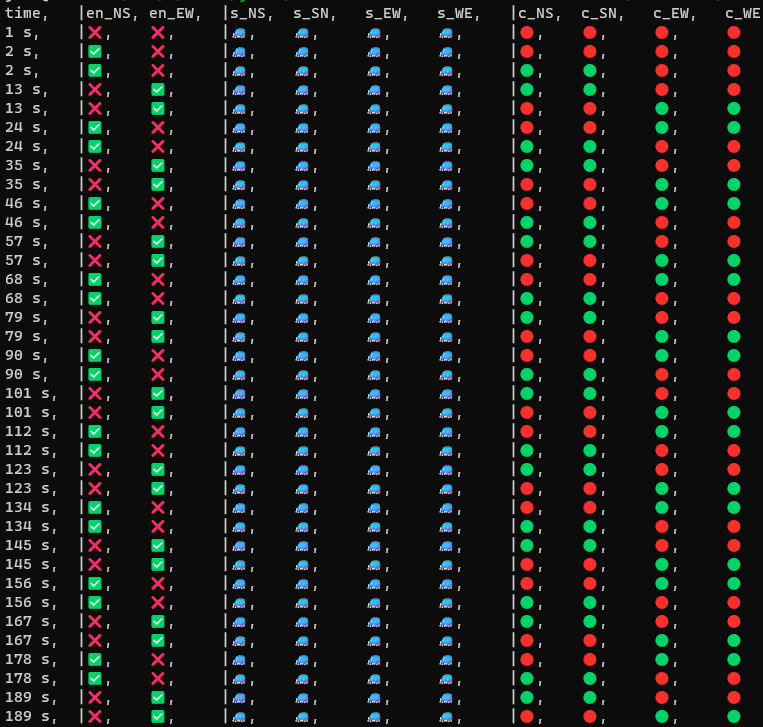
\includegraphics[width=34pc]{constant_traffic.png}}
    	\caption{Output after running the simulation for 200 seconds on constant stimuli.}
    	\label{fig:constant_traffic}
    \end{figure*}
    
    \paragraph*{No Traffic}
    Running the simulation on an input file which suggests that no cars are arriving the entire time, results in no events being triggered and hence an empty output file as desired (see Figure \ref{fig:no_traffic}).
    \begin{figure*}[H]
    	\centerline{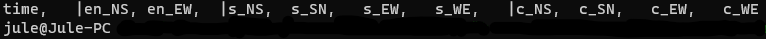
\includegraphics[width=34pc]{no_traffic.png}}
    	\caption{Output after running the simulation for 100 seconds on no stimuli.}
    	\label{fig:no_traffic}
    \end{figure*}
    
    \paragraph*{Randomly Generated Traffic}
    Finally, we tested the simulation with multiple randomly generated input files and verified our constraints by ensuring that the assertions do not fail. In Figure \ref{fig:independent_traffic} an output file illustrates the independent light behavior. In the boxes it can be seen that the lights are only turning green once the sensor reports a \texttt{1}. For example, a vehicle is waiting at sensor SN directly at the beginning, so that the traffic light for SN switches to green after one second. For sensor NS, on the other hand, the sensor does not report a \texttt{1} until second six. Therefore, the NS traffic light does not turn green until second six. 
    \begin{figure}[H]
    	\centerline{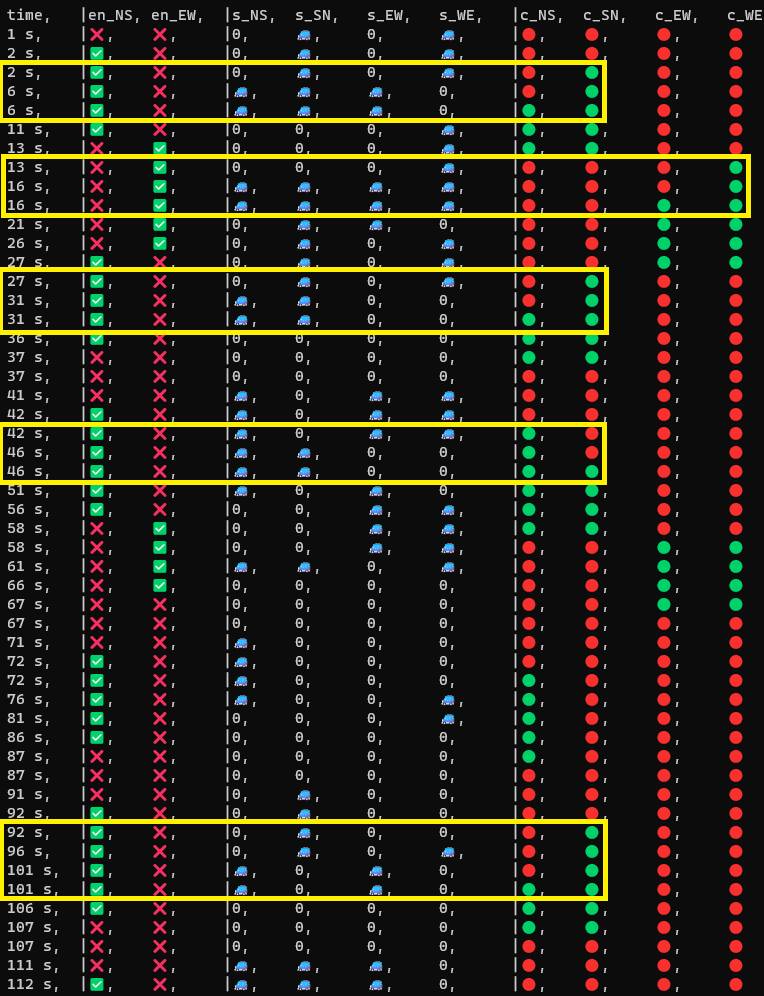
\includegraphics[width=34pc]{random_input_independence.png}}
    	\caption{Partial output screenshot after running the simulation on random input. Yellow boxes indicate the independent behavior of the traffic lights.}
    	\label{fig:independent_traffic}
    \end{figure}
    
    \paragraph*{Manual Explanation of a Test Case Simulation}
    Apart from checking the model via randomly generated input we created one input manually to check all of the testcases. The result can be seen in Figure \ref{fig:testcase_traffic}. It shows that the lights work independently as SN and NS as well as EW and WE are not always green at the same time. Moreover, the safety is ensured since the axes NS and EW are never enabled simultaneously. And finally, we can see that for arriving cars, there exists a mapping to green lights. Either at the same time if the axis is already enabled (see for example for cars in direction NS from 47 seconds to 51 seconds). Or the light turns green about 10 seconds later (e.g., cars arriving at EW around second 51 get green light at second 62).
    \begin{figure}[H]
    	\centerline{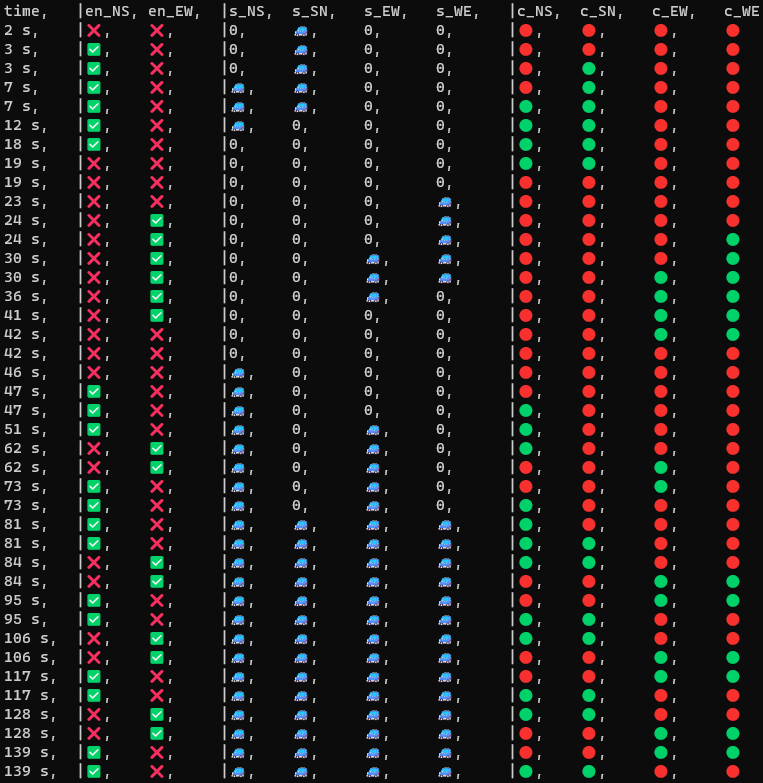
\includegraphics[width=34pc]{myTestcase_Output.png}}
    	\caption{Output after running the simulation on a test case input.}
    	\label{fig:testcase_traffic}
    \end{figure}
    


\section{Comment / Conclusion}
%Simon
\textit{simbu448}: I have seen that SystemC provides the tools to do RTL simulation as well as \textit{Functional Verification}. Having a background in VHDL, it was easy to adapt component instantiating, port maps and event driven processes with a sensitivity list in systemC.
When the assertions were completed, they were able to catch a flaw in the logic (Fig. \ref{fig:assertion_failed}). 
This exercise therefore showed an actual error in the programmed feature (Fig. \ref{fig:git_diff}) and thereby showing the importance of test driven development.
    
    \begin{figure}[H]
    	\centerline{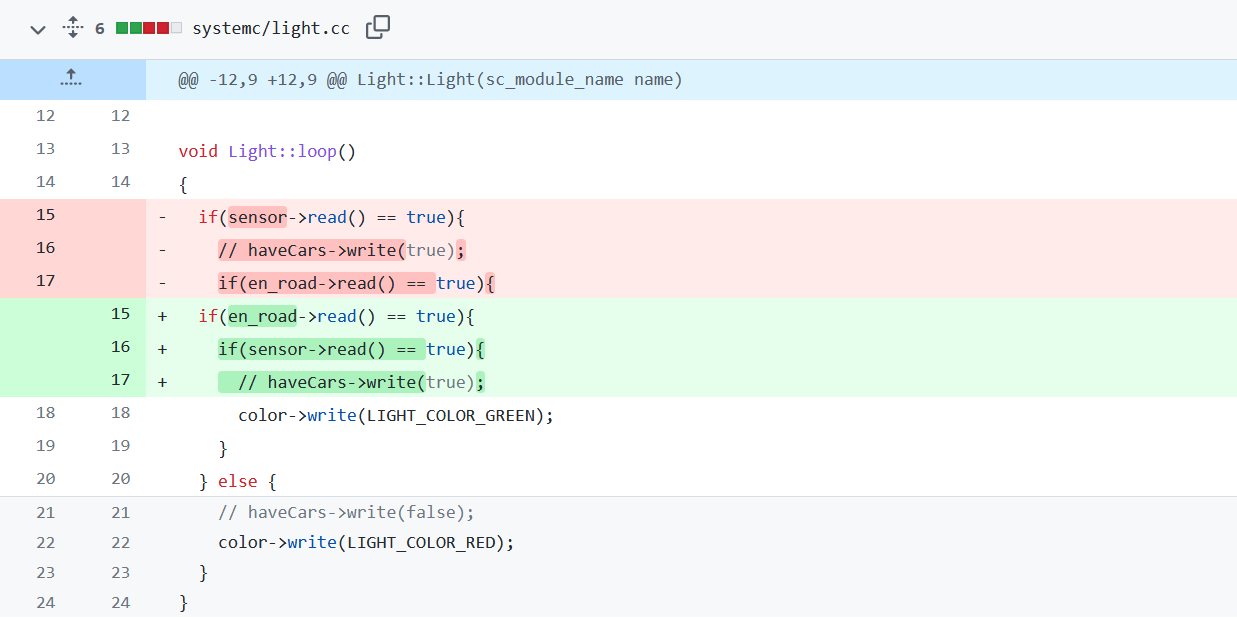
\includegraphics[width=34pc]{git_diff.png}}
    	\caption{The error was in the order of if-statements. There existed a case, when the light was not set to red when it should have.}
    	\label{fig:git_diff}
    \end{figure}
    

\end{document}
